\section{Synthesizing Optimizations}

For every cut extracted from an LLVM function, \minotaur{}'s goal is to
synthesize a cheaper way to compute the value returned by that cut.
%
It does this by enumerating \emph{candidates}---code fragments that
potentially refine the current cut.
%
When a candidate is found that refines the original cut, \minotaur{}
consults a cost model.
%
If the new code is cheaper than the original cut, \minotaur{} applies the
rewrite to the function that is being optimized.

\subsection{Designing an Appropriate Synthesis Procedure}

A delicate part of designing a practical program synthesis algorithm
is determining how much of the search is pushed to the solver, and how
much searching gets done by code outside the solver.
%
At one extreme, as the Denali paper~\cite{denali02} points out, we
could simply give the SMT solver a conjecture of the form ``No program
of the target architecture computes P in at most eight cycles.''
%
If the solver can disprove this conjecture, then its counterexample
will tell us how to compute P in eight or fewer cycles.
%
This kind of query is asking the solver to do all of the work of
finding a program that disproves the conjecture, including reasoning
about the costs of various alternatives, in a single, complicated
query---this is very heavy lifting.
%
At the other extreme, we could enumerate completely concrete
candidates, and use the SMT solver only to perform the necessary
refinement checks.
%
The problem with this approach is literal constants: even a single
64-bit constant in the synthesized code will require us to enumerate
and check $2^{64}$ alternatives; this is clearly infeasible.


We spent a considerable amount of time investigating different points
between these extremes, and finally settled on a design that makes
things as easy as possible for the solver, but without exploring all
possible choices of values for literal constants.
%
\minotaur{} creates \emph{partially symbolic} candidates where
instructions are represented concretely, but constants are symbolic.
%
This gives a reasonably tractable enumeration space without giving up
synthesis power.
%
Our rationale for this design is that, based on extensive experience
with LLVM and Alive2, a lot of individual refinement checks that we
want to perform---especially those that contain multiplications,
divisions, floating point operations, and pointer indirections---are
already very difficult.


\subsection{Synthesis in Minotaur}

\begin{table}[tbp]
  \centering
  \caption{Operations that \minotaur{} can synthesize.}
  \begin{tabular}{ r | l }
    \textbf{Operation Type} & \textbf{Instructions} \\
    \hline
    Unary integer & ctpop, ctlz, cttz, bitreverse, bswap \\
    Unary FP & fneg, fabs, fceil, ffloor, frint, fround, fnearbyint, froundeven \\
    Binary integer & add, sub, mul, udiv, sdiv, umax, umin, smax, smin\\
    Binary FP & fadd, fsub, fmul, fdiv, frem, fmaximum, fminimum, ... \\
    Bitwise & and, or, xor, shl, lshr, ashr \\
    Comparison & icmp, fcmp, select \\
    Conversion & zext, sext, trunc, fptrunc, fpext, fptosi, sitofp, fptoui, uitofp \\
    Data movement & extractelement, insertelement, shufflevector \\
    SIMD intrinsics & 165 vector intrinsics mapping to intel vector instructions \\
  \end{tabular}
  \label{tab:operations}
\end{table}

\begin{algorithm}[tbp]
  \caption{Minotaur's Synthesis Procedure.}
  \label{alg:enumerate}
  \begin{algorithmic}[1]
  \Function{SynthesizeRefinements}{Cut: Function, InstLimit: $\mathbb{N}$, TimeLimit: $\mathbb{N}$}


  \State {Inputs $\gets$ all the SSA definitions in Cut}
  \State{InstPool $\gets \emptyset$}
  \ForAll {op in binary operations listed in Table~\ref{tab:operations}}
    \State {InstPool $\gets$ InstPool $\cup$ \{ (op hole, hole), (op sym-const, hole)\} }
    \ForAll {input1 in Inputs}
      \State {InstPool $\gets$ InstPool $\cup$ \{ (op input1, sym-const), (op sym-const, input1) \}}
      \State {InstPool $\gets$ InstPool $\cup$ \{ (op input1, hole), (op hole, input1) \}}
      \ForAll {input2 in Inputs}
        \State {InstPool $\gets$ InstPool $\cup$ \{ (op input1, input2) \}}
      \EndFor
    \EndFor
  \EndFor

  \ForAll {other operations in Table~\ref{tab:operations}}
  \Comment{omitted for brevity}
    \State {...}
  \EndFor

  \State {WorkList $\gets$ \{ (ret hole), (ret sym-const) \} }

  \State {Candidates $\gets$ Inputs}

  \While {WorkList $\neq \emptyset$}
    \State {I $\gets$ WorkList.pop()}

    \If {I does not contain holes}
      \State {Candidates $\gets$ Candidates $\cup$ \{ I \}}
      \State{\textbf{continue}}
    \EndIf

    \ForAll {Hole in I}
      \If {CountNewInsts(I) $\geq$ InstLimit}
        \State{\textbf{continue}}
      \EndIf
      \ForAll {Inst in InstPool}
        \State {J $\gets$ I with Hole substituted by Inst}
          \If {TargetTransformInfoCost(J) $\geq$ TargetTransformInfoCost(Cut)}
            \State{\textbf{continue}}
          \EndIf

          \State {WorkList $\gets$ WorkList $\cup$ \{ J \}}
      \EndFor
    \EndFor

  \EndWhile

  \State {Sort Candidates by TargetTransformInfoCost}
  \State {StartTime $\gets$ time()}
  \State {Refinements $\gets \emptyset$}

  \ForAll {C in Candidates}
    \If {C does not contain symbolic constants}
      \If {Alive2 claims that C refines Cut}
        \State {Refinements $\gets$ Refinements $\cup$ \{ C \}}
      \EndIf
    \Else
      \State {Build exists-forall query to get a model for symbolic constants}
      \If {satisfiable}
        \State {C' $\gets$ C with constants substituted by the constants in the model}
        \State {Refinements $\gets$ Refinements $\cup$ \{ C' \}}
      \EndIf
    \EndIf
    \If {time() - StartTime $\geq$ TimeLimit}
      \State{\textbf{break}}
    \EndIf
  \EndFor

  \State{\textbf{return} Refinements}

  \EndFunction
  % \State{\{ Complete, Incomplete \} $\gets$ \textsc{GenerateSingleInstruction}(Inputs)}
  % \State {WiredInsts $\gets$ Put Complete and Incomplete into the each of holes in Inst}
  \end{algorithmic}
  \label{alg:synthesis}
\end{algorithm}

Algorithm~\ref{alg:synthesis} describes \minotaur's synthesis procedure.
%
In Phase~1, it creates a pool of instructions whose operands are
selected from the available SSA values in the current cut (a dominance
check is not required since cuts are constructed in such a way that
every existing SSA definition dominates the synthesized portion of the
function), from symbolic constants, and from \emph{holes} that
represent instructions that have not yet been enumerated.
%
The list of instructions that \minotaur{} can synthesize is shown in
Table~\ref{tab:operations}.
%
The description in Algorithm~\ref{alg:synthesis} only shows the case
for instructions taking two operands, and it also omits a number of
simple pruning strategies that are useful in practice, such as
avoiding enumeration of redundant versions of commutative operations.
%
In Phase~2 of the synthesis procedure, instructions from the pool are
used to recursively fill holes; this procedure terminates when all
holes are filled (in which case a complete candidate has been
generated) or when at least one hole remains, but there is no remaining
instruction budget to fill it (in which case the incomplete candidate
is discarded).
%
A subtlety here is that
LLVM's \texttt{bitcast} instruction, which changes the type
of an SSA value without changing its representation, does not count
towards the instruction limit.
%
This is because \minotaur{} takes a low-level, untyped view of values.
%
For example, it internally treats a 16-way vector of 8-bit values the
same as an 8-way vector of 16-bit values: both of these are simply
128-bit quantities.
%
This lack of type enforcement allows \minotaur{} to find interesting,
low-level optimizations such as those that use bitwise operations to
rapidly perform certain floating point operations.


\begin {figure}[tbp]
  \centering
  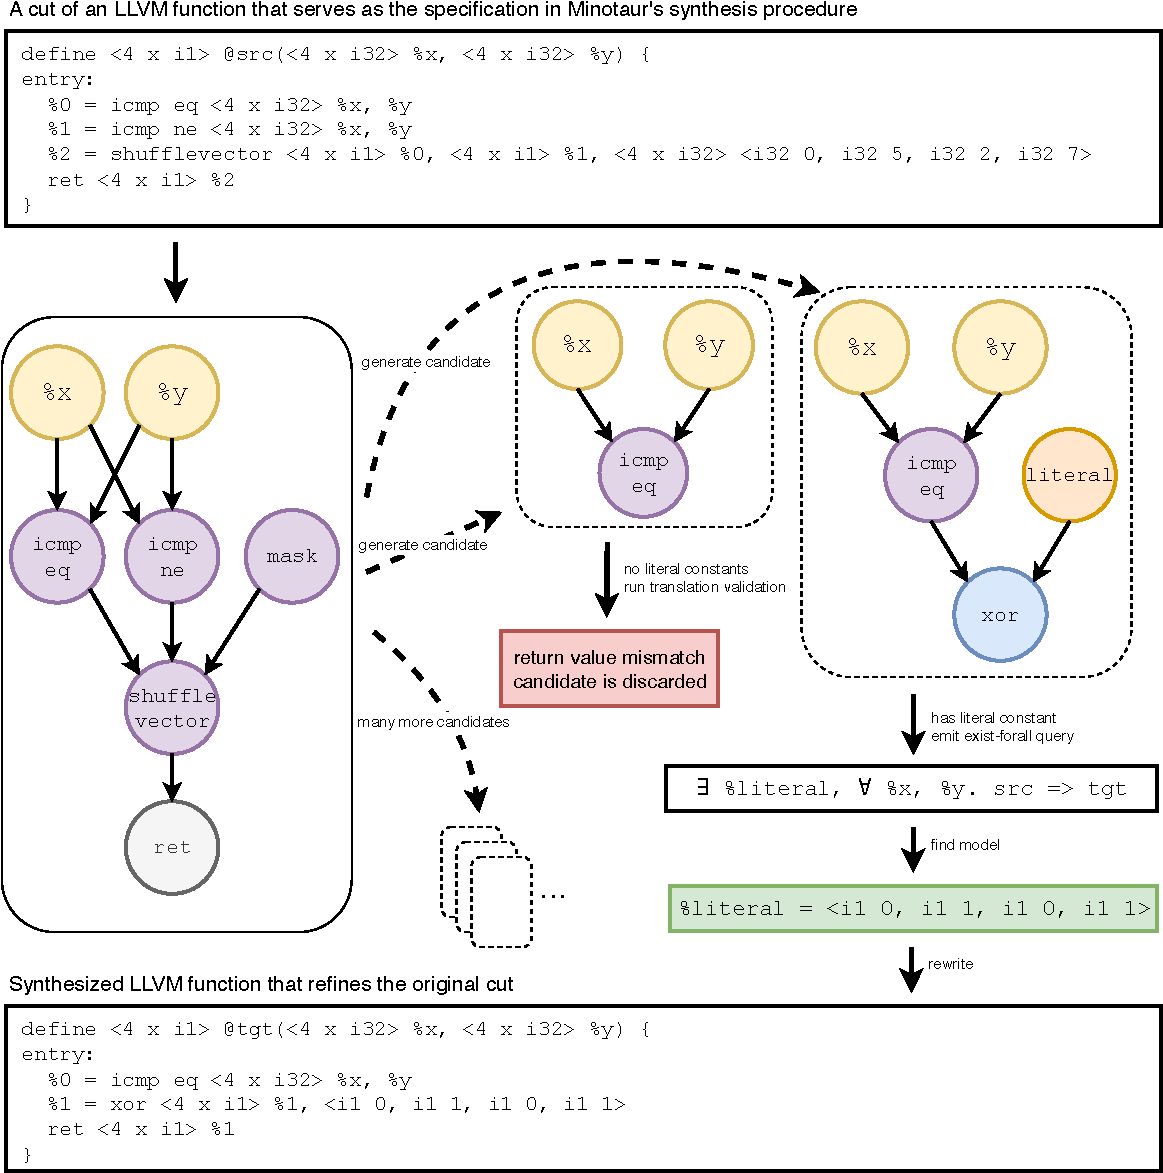
\includegraphics[width=0.8\linewidth]{figures/solve_literal.pdf}
  \caption{Example of synthesizing a rewrite that contains literal constants.}
  \label{fig:synthesizing}
\end{figure}

In Phase~3 of Algorithm~\ref{alg:synthesis}, \minotaur{} uses Alive2 to
eliminate every candidate that does not refine the specification.
%
First, we sort the candidates in order of increasing cost using LLVM's
TargetTransformInfo~\cite{tti}: a cost model that roughly captures
execution cost on the target, and is cheap to compute.
%
We do this to ensure that likely-beneficial rewrites are tested first,
before the synthesis time limit is reached.
%
For candidates that do not contain symbolic constants, we can use
Alive2 as-is.
%
To support symbolic constants, we modified Alive2 to wrap
its refinement check in an exists-forall query.
%
In other words, \minotaur{} asks the question: ``Does there exist a
valuation of the symbolic constants such that the synthesis candidate
refines the specification for all possible values of the inputs?''
%
When such a query is satisfiable, the model returned by the solver can
be inspected to find satisfying values of the symbolic constants
in the candidate, which now become literal constants, giving a
complete, sound optimization.
%
To avoid potentially-expensive exists-forall queries, we experimented
with various techniques such as generalization by
substitution~\cite{Dutertre15}.
%
However, these failed to outperform exists-forall queries, in the
version of Z3 that we used (4.12.4).
%
Figure~\ref{fig:synthesizing} illustrates \minotaur's synthesis procedure.


\subsection{Identifying Profitable Rewrites}

The output of Algorithm~\ref{alg:synthesis} is a list of candidates
that all refine the cut.
%
Of these, we want to choose the best one---but predicting throughput
of code running on modern microprocessors is not straightforward.
%
We leverage the LLVM Machine Code Analyzer (LLVM-MCA)~\cite{llvmmca},
which was created to help developers improve performance-critical
code.
%
It is an interactive tool that emits a graphical depiction of pipeline
behavior, but its functionality can also be accessed programmatically,
and this is what \minotaur{} does, after lowering each candidate to
x86-64 object code.
%
Then, \minotaur{} only applies a rewrite if its estimated cost, using
LLVM-MCA, is lower than that of the original cut, and lower than
that of any other synthesized refinement of the original cut.


Although LLVM-MCA can estimate the cycle cost of LLVM functions, we
instead use the number of uOps (``micro-operations,'' a modern x86-64
processor's internal instruction set) as the estimated cost.
%
This choice was driven by empirical data: after extensive
experimentation, we determined that, for our purposes, uOps are a
better performance predictor than cycles.



\subsection{Representing and Caching Rewrites}
\label{sec:rewrite}

\minotaur{} stores each potential rewrite as a pair: $(C, S)$
where $C$ is a cut, represented by a function in LLVM
Intermediate Representation (IR), and $S$ is a rewrite description---an
expression in \minotaur's own intermediate representation that describes a
different way to compute the return value of $C$.
%
Rewrite descriptions are directed acyclic graphs containing nodes that represent
operations, and edges representing data flow.
%
Although the elements found in \minotaur{} IR are similar to those found
in LLVM IR, we could not reuse LLVM IR to represent rewrites since
LLVM IR does not support incomplete code fragments, and also rewrites
must contain enough information to support connecting the new code in
the rewrite to code in the unoptimized function.


To support caching, rewrites must be serializable.
%
The cut $C$ can be serialized using existing LLVM functionality, and we
created a simple S-expression syntax for serializing the $S$ part.
%
Figure~\ref{fig:syntax} shows the syntax of the IR\@.
%
For example, if the returning value of $C$, a 32-bit instruction is
replaced by left shift by one bit position, the textual format for
the expression is \texttt{(shl (val i32 \%0), (const i32 1), i32)}.


Rewrites are cached in a Redis instance: this implementation choice
allows the cache to be persistent across multiple \minotaur{} runs and
also makes the cache network-accessible.
%
Synthesis can be done online---during compilation---but also
offline, in a mode where \minotaur{} extracts cuts into the Redis
cache but does not perform synthesis.
%
In this mode, compilation is only slowed down by a few percent.
%
\minotaur's offline mode is designed for batch processing.
%
In this mode, a separate program called \texttt{cache-infer} retrieves
cuts from the cache, runs synthesis on them, and stores any
optimizations that it discovers back into the cache.
%
Unlike the online mode, which runs synthesis tasks one after the
other, offline mode can run all synthesis jobs in parallel.



\begin{figure}[tbp]
  \begin{tabular}{r c l}
    \emph{Op} &::=& \emph{Inst} $|$ \emph{Constant} $|$ \emph{Value} \\
    \emph{Inst}  &::=& (\emph{UnaryOp} \emph{Op}, \emph{Type}) $|$ (\emph{BinaryOp} \emph{Op}, \emph{Op}, \emph{Type}) $|$   \\
              && (insertelement \emph{Op}, \emph{Op}, \emph{Op}) $|$  (extractelement \emph{Op}, \emph{Op}) $|$ \\
              && (shufflevector \emph{Op}, \emph{Op}, \emph{Constant}) $|$ (\emph{Conversion} \emph{Op}, \emph{Type}) $|$\\
              && (\emph{Comparison} \emph{Op} \emph{Op}) $|$  (select \emph{Op}, \emph{Op}, \emph{Op}) $|$  (\emph{Intrinsic} \emph{Op}, \emph{Op}) \\
    \emph{Constant} &::=& (const \emph{Type} \texttt{number-literal}) \\
    \emph{Value} &::=& (val \emph{Type} \texttt{llvm-identifier}) \\

    \emph{Type} &::=& \emph{ScalarType} $|$  <elements $\times$ \emph{ScalarType}> \\
    \emph{ScalarType} &::=& i1 $|$  i8 $|$  i16 | i32 $|$  i64 $|$  half $|$  float $|$  double $|$  fp128 \\
    \emph{BinaryOp} &::=& xor $|$  and $|$  or $|$  add $|$  sub $|$  mul $|$  udiv $|$  sdiv $|$  ashr $|$   \\
                 && lshr $|$  shl $|$  umax $|$  umin $|$  smax $|$  smin\\
                && fadd $|$  fsub $|$  fmul $|$  fdiv $|$ copysign $|$ \\
                &&    fmaximum $|$  fminimum $|$  fmaxnum $|$  fminnum \\
    \emph{UnaryOp} &::=& ctpop $|$  ctlz $|$  cttz $|$  bswap $|$  bitreverse $|$ fneg $|$  fabs $|$  fceil $|$ \\
                      &&   ffloor $|$  frint $|$  fround $|$  ftrunc $|$  fnearbyint $|$  froundeven \\
    \emph{Conversion} &::=& zext $|$  sext $|$  trunc $|$ \\
                    && fptrunc $|$  fpext $|$  fptosi $|$  sitofp $|$  fptoui $|$  uitofp \\
    \emph{Comparison} &::=& eq $|$  ne $|$  ult $|$  ule $|$  slt $|$  sle $|$ \\
                && oeq $|$  ogt $|$  oge $|$  olt $|$  ole $|$  one $|$  ord $|$ \\
                && ueq $|$  ugt $|$  uge $|$  ult $|$  ule $|$  une $|$  uno \\
    \emph{Intrinsic} &::=&  avx2.pavg.b $|$  avx512.pmaddubs.w.512 $|$  \dots (165 intrinsics in total) \\
  \end{tabular}
  \caption{Syntax for \minotaur{} rewrites.}
  \label{fig:syntax}
  %\Description[syntax]{Minotaur syntax}
\end{figure}



\subsection{Integration with LLVM}

\minotaur{} is loaded into LLVM as a shared library where it runs as an
optimization pass.
%
We arranged for it to run at the end of LLVM's auto-vectorization pipeline.
%
We invoke LLVM's Dead Code Elimination pass after Minotaur to
clean up the resulting code.
